\documentclass[man,floatsintext]{apa6}
\usepackage{lmodern}
\usepackage{amssymb,amsmath}
\usepackage{ifxetex,ifluatex}
\usepackage{fixltx2e} % provides \textsubscript
\ifnum 0\ifxetex 1\fi\ifluatex 1\fi=0 % if pdftex
  \usepackage[T1]{fontenc}
  \usepackage[utf8]{inputenc}
\else % if luatex or xelatex
  \ifxetex
    \usepackage{mathspec}
  \else
    \usepackage{fontspec}
  \fi
  \defaultfontfeatures{Ligatures=TeX,Scale=MatchLowercase}
\fi
% use upquote if available, for straight quotes in verbatim environments
\IfFileExists{upquote.sty}{\usepackage{upquote}}{}
% use microtype if available
\IfFileExists{microtype.sty}{%
\usepackage{microtype}
\UseMicrotypeSet[protrusion]{basicmath} % disable protrusion for tt fonts
}{}
\usepackage{hyperref}
\hypersetup{unicode=true,
            pdftitle={Our APA document for Lab 8},
            pdfauthor={Cameron S. Kay, Stefania R. Ashby, \& Ashley L. Miller},
            pdfkeywords={apa, papaja, science},
            pdfborder={0 0 0},
            breaklinks=true}
\urlstyle{same}  % don't use monospace font for urls
\usepackage{graphicx,grffile}
\makeatletter
\def\maxwidth{\ifdim\Gin@nat@width>\linewidth\linewidth\else\Gin@nat@width\fi}
\def\maxheight{\ifdim\Gin@nat@height>\textheight\textheight\else\Gin@nat@height\fi}
\makeatother
% Scale images if necessary, so that they will not overflow the page
% margins by default, and it is still possible to overwrite the defaults
% using explicit options in \includegraphics[width, height, ...]{}
\setkeys{Gin}{width=\maxwidth,height=\maxheight,keepaspectratio}
\IfFileExists{parskip.sty}{%
\usepackage{parskip}
}{% else
\setlength{\parindent}{0pt}
\setlength{\parskip}{6pt plus 2pt minus 1pt}
}
\setlength{\emergencystretch}{3em}  % prevent overfull lines
\providecommand{\tightlist}{%
  \setlength{\itemsep}{0pt}\setlength{\parskip}{0pt}}
\setcounter{secnumdepth}{0}
% Redefines (sub)paragraphs to behave more like sections
\ifx\paragraph\undefined\else
\let\oldparagraph\paragraph
\renewcommand{\paragraph}[1]{\oldparagraph{#1}\mbox{}}
\fi
\ifx\subparagraph\undefined\else
\let\oldsubparagraph\subparagraph
\renewcommand{\subparagraph}[1]{\oldsubparagraph{#1}\mbox{}}
\fi

%%% Use protect on footnotes to avoid problems with footnotes in titles
\let\rmarkdownfootnote\footnote%
\def\footnote{\protect\rmarkdownfootnote}


  \title{Our APA document for Lab 8}
    \author{Cameron S. Kay\textsuperscript{1}, Stefania R. Ashby\textsuperscript{1},
\& Ashley L. Miller\textsuperscript{1}}
    \date{}
  
\shorttitle{Lab 8 APA document}
\affiliation{
\vspace{0.5cm}
\textsuperscript{1} University of Oregon}
\keywords{apa, papaja, science}
\usepackage{csquotes}
\usepackage{upgreek}
\captionsetup{font=singlespacing,justification=justified}

\usepackage{longtable}
\usepackage{lscape}
\usepackage{multirow}
\usepackage{tabularx}
\usepackage[flushleft]{threeparttable}
\usepackage{threeparttablex}

\newenvironment{lltable}{\begin{landscape}\begin{center}\begin{ThreePartTable}}{\end{ThreePartTable}\end{center}\end{landscape}}

\makeatletter
\newcommand\LastLTentrywidth{1em}
\newlength\longtablewidth
\setlength{\longtablewidth}{1in}
\newcommand{\getlongtablewidth}{\begingroup \ifcsname LT@\roman{LT@tables}\endcsname \global\longtablewidth=0pt \renewcommand{\LT@entry}[2]{\global\advance\longtablewidth by ##2\relax\gdef\LastLTentrywidth{##2}}\@nameuse{LT@\roman{LT@tables}} \fi \endgroup}


\DeclareDelayedFloatFlavor{ThreePartTable}{table}
\DeclareDelayedFloatFlavor{lltable}{table}
\DeclareDelayedFloatFlavor*{longtable}{table}
\makeatletter
\renewcommand{\efloat@iwrite}[1]{\immediate\expandafter\protected@write\csname efloat@post#1\endcsname{}}
\makeatother

\authornote{

Correspondence concerning this article should be addressed to Cameron S.
Kay, 1451 Onyx Street, Eugene, OR 97403. E-mail:
\href{mailto:ckay@uoregon.edu}{\nolinkurl{ckay@uoregon.edu}}}

\abstract{
Here is an abstract. It is abstract but also specific.


}

\begin{document}
\maketitle

I am writing an introduction. Caprara, Barbaranelli, Steca, and Malone
(2006) found some stuff. But other people have found other stuff
(Zimmerman, 1990).

\newpage

\section{Methods}\label{methods}

We report how we determined our sample size, all data exclusions (if
any), all manipulations, and all measures in the study.

\subsection{Participants}\label{participants}

\subsection{Material}\label{material}

\subsection{Procedure}\label{procedure}

\subsection{Data analysis}\label{data-analysis}

\newpage

\section{Results}\label{results}

As shown in Table 1, the mean math and reading scores for boys with
\enquote{yes} for frl was lower than the mean math and reading scores
for boys with \enquote{no} for frl. In contrast, the mean math and
reading scores for girls with \enquote{yes} for frl was higher than the
mean math and reading scores for girls with \enquote{no} for frl. For
both levels of frl, the mean math and reading scores were higher for
girls than boys.

\begin{table}[h]
\begin{center}
\begin{threeparttable}
\caption{\label{tab:create_table}Descriptive statistics for math and reading, grouped by sex and frl.}
\begin{tabular}{llllll}
\toprule
sex & \multicolumn{1}{c}{frl} & \multicolumn{1}{c}{math\_mean} & \multicolumn{1}{c}{math\_sd} & \multicolumn{1}{c}{rdg\_mean} & \multicolumn{1}{c}{rdg\_sd}\\
\midrule
boy & no & 492.85 & 46.34 & 441.46 & 32.32\\
boy & yes & 469.87 & 46.09 & 425.38 & 26.63\\
girl & no & 501.21 & 45.96 & 448.54 & 34.52\\
girl & yes & 477.51 & 46.30 & 430.80 & 27.42\\
\bottomrule
\end{tabular}
\end{threeparttable}
\end{center}
\end{table}

As shown in Figure 1, there is a similar relationship between teacher
experience and student performance on math for both groups of students.
With more years of teaching experience, students do better on their math
scores. However students who receive free/reduced priced meals (implying
lower socioeconomic status) have an overall deficit compared to students
with higher socioeconomic status, demonstrating that they are at a
disadvantage from the beginning.

\begin{figure}
\centering
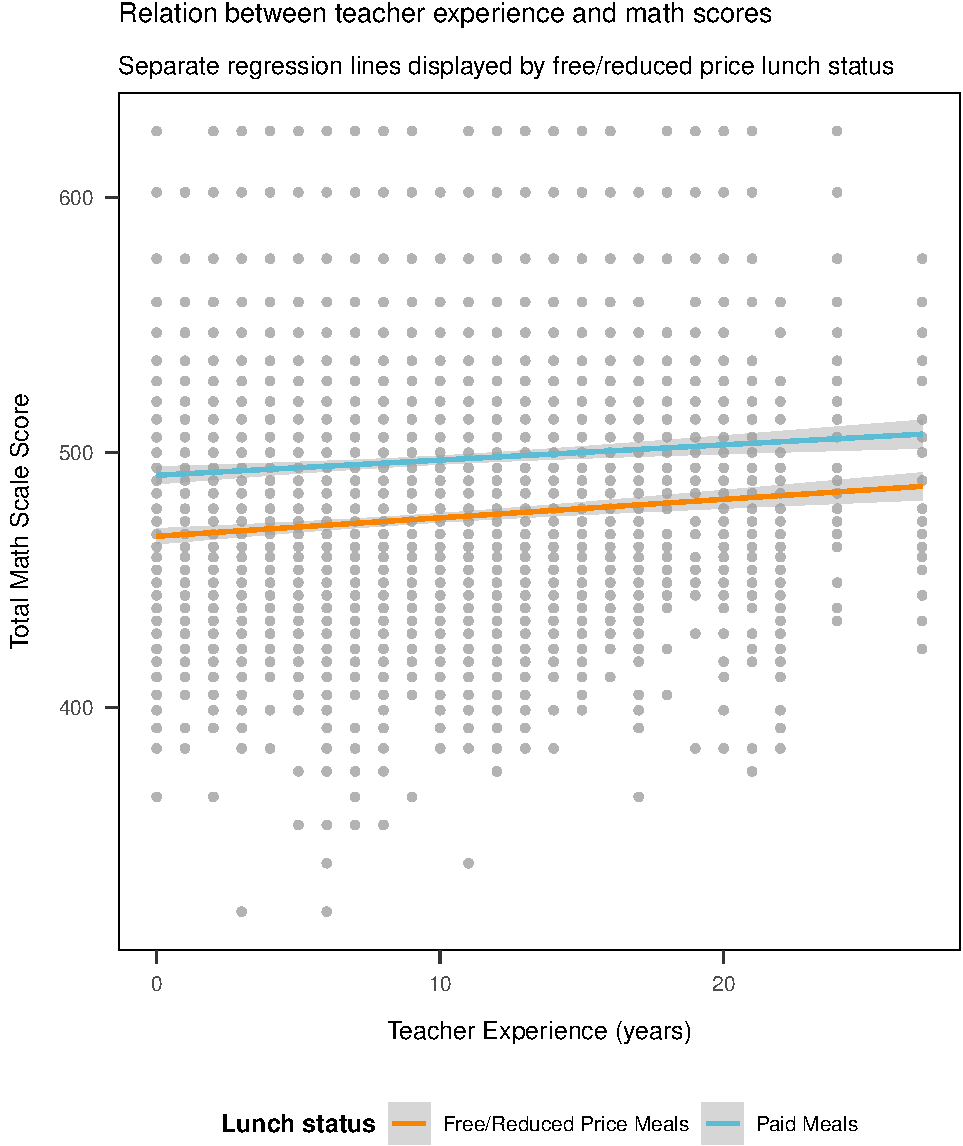
\includegraphics{lab_8_apa_document_files/figure-latex/create plot-1.pdf}
\caption{}
\end{figure}

\newpage

\section{Discussion}\label{discussion}

\newpage

\section{References}\label{references}

\begingroup
\setlength{\parindent}{-0.5in} \setlength{\leftskip}{0.5in}

\hypertarget{refs}{}
\hypertarget{ref-caprara2006teachers}{}
Caprara, G. V., Barbaranelli, C., Steca, P., \& Malone, P. S. (2006).
Teachers' self-efficacy beliefs as determinants of job satisfaction and
students' academic achievement: A study at the school level.
\emph{Journal of School Psychology}, \emph{44}, 473--490.

\hypertarget{ref-zimmerman1990self}{}
Zimmerman, B. J. (1990). Self-regulated learning and academic
achievement: An overview. \emph{Educational Psychologist}, \emph{25},
3--17.

\endgroup


\end{document}
